%%%%%%%%%%%%%%%%%%%%%%%%%%%%%%%%%%%%%%%%%%%%%%%%%%%%%%%%%%%%%%%%%%%%%%%%%%%
%%%                                                                     %%%
%%%   LaTeX template voor het verslag van P&O: Computerwetenschappen.   %%%
%%%                                                                     %%%
%%%   Opties:                                                           %%%
%%%     tt      Tussentijdsverslag                                      %%%
%%%     eind    Eindverslag                                             %%%
%%%                                                                     %%%
%%%   7 februari 2014                                                   %%%
%%%   Versie 1.2                                                        %%%
%%%                                                                     %%%
%%%%%%%%%%%%%%%%%%%%%%%%%%%%%%%%%%%%%%%%%%%%%%%%%%%%%%%%%%%%%%%%%%%%%%%%%%%

\documentclass[tt]{penoverslag}

%%% PACKAGES %%%
\usepackage{graphicx}
\usepackage{amsmath}
\usepackage{wasysym}
\usepackage{float}
\usepackage{wrapfig}
\setlength\parindent{0pt}

\begin{document}

% == TITELPAGINA == %
\team{Indigo} % teamkleur
\members{
        Wander Bavin\\
        Vince Goossens\\
        Dimitri Jonckers\\
        Sunil Tandan\\
        Wout Vekemans} % teamleden
\maketitlepage


% == SAMENVATTING == %
\begin{abstract}
\noindent
Dit rapport documenteert onze analyse en oplossing van het volgende probleem : de constructie en operatie van een zeppelin in wedstrijdverband. De zeppelin maakt gebruik van een gekend grondplan in roostervorm voor navigatie. De positie van de zeppelin wordt bepaald door een algoritme gebaseerd op beeldherkenning. Via het rooster moet hij sneller dan een andere zeppelin naar een bepaalde positie vliegen, en een andere, nog onbekende opdracht uitvoeren. Beide zeppelins dienen met een RabbitMQ-server te communiceren om informatie uit te wisselen met hun sturende laptop, en met elkaar. Een GUI dient de toestand van het speelveld met beide zeppelins te visualiseren. Al deze functionaliteiten worden ge\"{i}mplementeerd in Java. Op dit moment staan alle delen van de software nog in de steigers, maar werkende functies zijn niet veraf.
\end{abstract}


% == INHOUDSOPGAVE == %
\tableofcontents\newpage


% == INLEIDING == %
\section{Inleiding}
Dit tweede deel van de bachelorproef draait nog steeds rond het aansturen van een zeppelin op basis van een Raspberry Pi. 

\paragraph{Fysisch ontwerp}
~\\
De zeppelin bestaat uit een houten frame waaraan 2 heliumballonnen ($\diameter$90 cm) vastgemaakt zijn. Aan het frame zijn een camera en een afstandssensor vastgemaakt, die beiden naar beneden gericht zijn. Zowel de camera als de afstandssensor zijn verbonden met een Raspberry Pi die in het frame zit ingebed. Het geheel bevat drie propellers: twee voor horizontale bewegingen en \'{e}\'{e}n voor verticale bewegingen.


\paragraph{Software ontwerp}
~\\
De software die inwendig op de Pi draait en op de client-pc voor image processing en weergave van de GUI is geschreven in Java. De communicatie tussen de zeppelin en de client gebeurt via een server. (Zie figuur \ref{schema}). \\

TODO !!!! schema figuur
\begin{figure}[ht!]
\centering
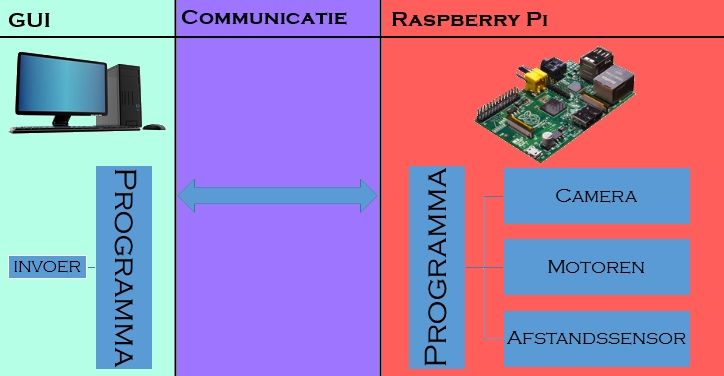
\includegraphics[height=55mm]{Schema.jpg}
\caption{Architectuur}
\label{schema}
\end{figure}

% == Beschrijving materiaal en bouw zeppelin == %
\section{Beschrijving materiaal en bouw zeppelin}
De zeppelin bestaat uit een frame waaraan alle onderdelen zijn vastgemaakt. Hierop worden onder andere de 3 propellers bevestigd. Twee hiervan dienen om naar links en rechts te draaien. Om vooruit te bewegen worden deze samen geactiveerd met dezelfde kracht. Deze propellers bevinden zich aan de uiteindes van de vleugels. De derde propeller, om de zeppelin te laten stijgen, is naar beneden gericht. De propellers kunnen op volle kracht of door middel van pwm\footnote{en.wikipedia.org/wiki/Pulse-width\_modulation} worden aangestuurd (in 2 richtingen). Met deze techniek is het mogelijk om naast de richting ook de kracht van de motor in te stellen. Het is slechts mogelijk om \'e\'en propeller aan te sturen met pwm. We hebben hiervoor de motor voor verticale bewegingen genomen. Zo is het mogelijk de hoogte accuraat te regelen. ~\\

\begin{figure}[h!]
\centering
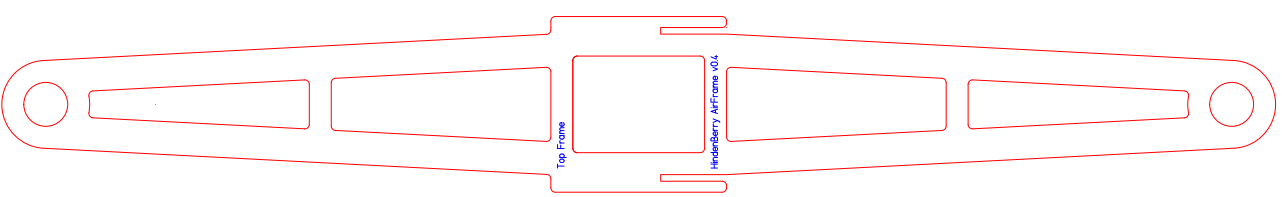
\includegraphics[scale=0.3]{upperFrame.png}
\label{frame}
\end{figure}

\begin{figure}[h!]
\centering
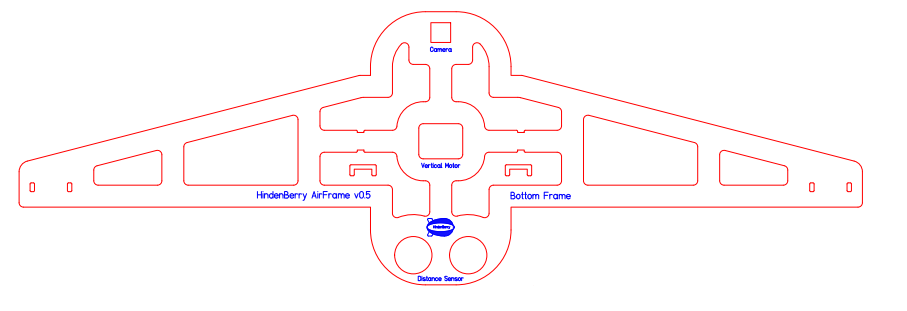
\includegraphics[scale=0.3]{lowerFrame.png}
\caption{Blueprint van het frame}
\label{frame}
\end{figure}

Om het geheel in de lucht te houden, zitten er 2 heliumballonnen ($\diameter$90 cm) vast aan de bovenkant van het frame. Deze hebben initieel een lift van 268 gr per stuk, maar dit vermindert wanneer de ballonnen doorheen de weken volume verliezen. \\

De zeppelin wordt aangestuurd door een Raspberry Pi model A. Deze heeft volgende specificaties:
\begin{itemize}
\item \emph{Processor:} 700MHz ARM
\item \emph{Geheugen:} 256MB
\item \emph{Poorten:} 1 USB 2.0, HDMI, audio out, RCA video
\item \emph{Voeding:} Micro USB
\item GPIO-pinnen om de hardware aan te sturen
\end{itemize}

In de Raspberry Pi zit een SD-kaart van 4 GB. Hierop staat Raspbian, het standaard besturingssysteem van de Raspberry Pi. Er is nog voldoende ruimte over om onze eigen programma's als jar-file op de Pi te zetten. \\

Verder zijn er nog 2 devices waarvan de zeppelin gebruik maakt:
\begin{itemize}
\item \emph{De camera} laat toe foto's te nemen met een maximum resolutie van 5 MP. Hiermee kunnen we onder andere beelden maken van QR-codes. Daarnaast kan de camera video's maken met resoluties tot 1080p.
\item \emph{De afstandssensor} kan worden gebruikt om met ultrasone trillingen de afstand te meten tussen de zeppelin en de grond of muur. Het bereik gaat van 2-400 cm. \\
\end{itemize}

\begin{figure}[ht!]
\centering
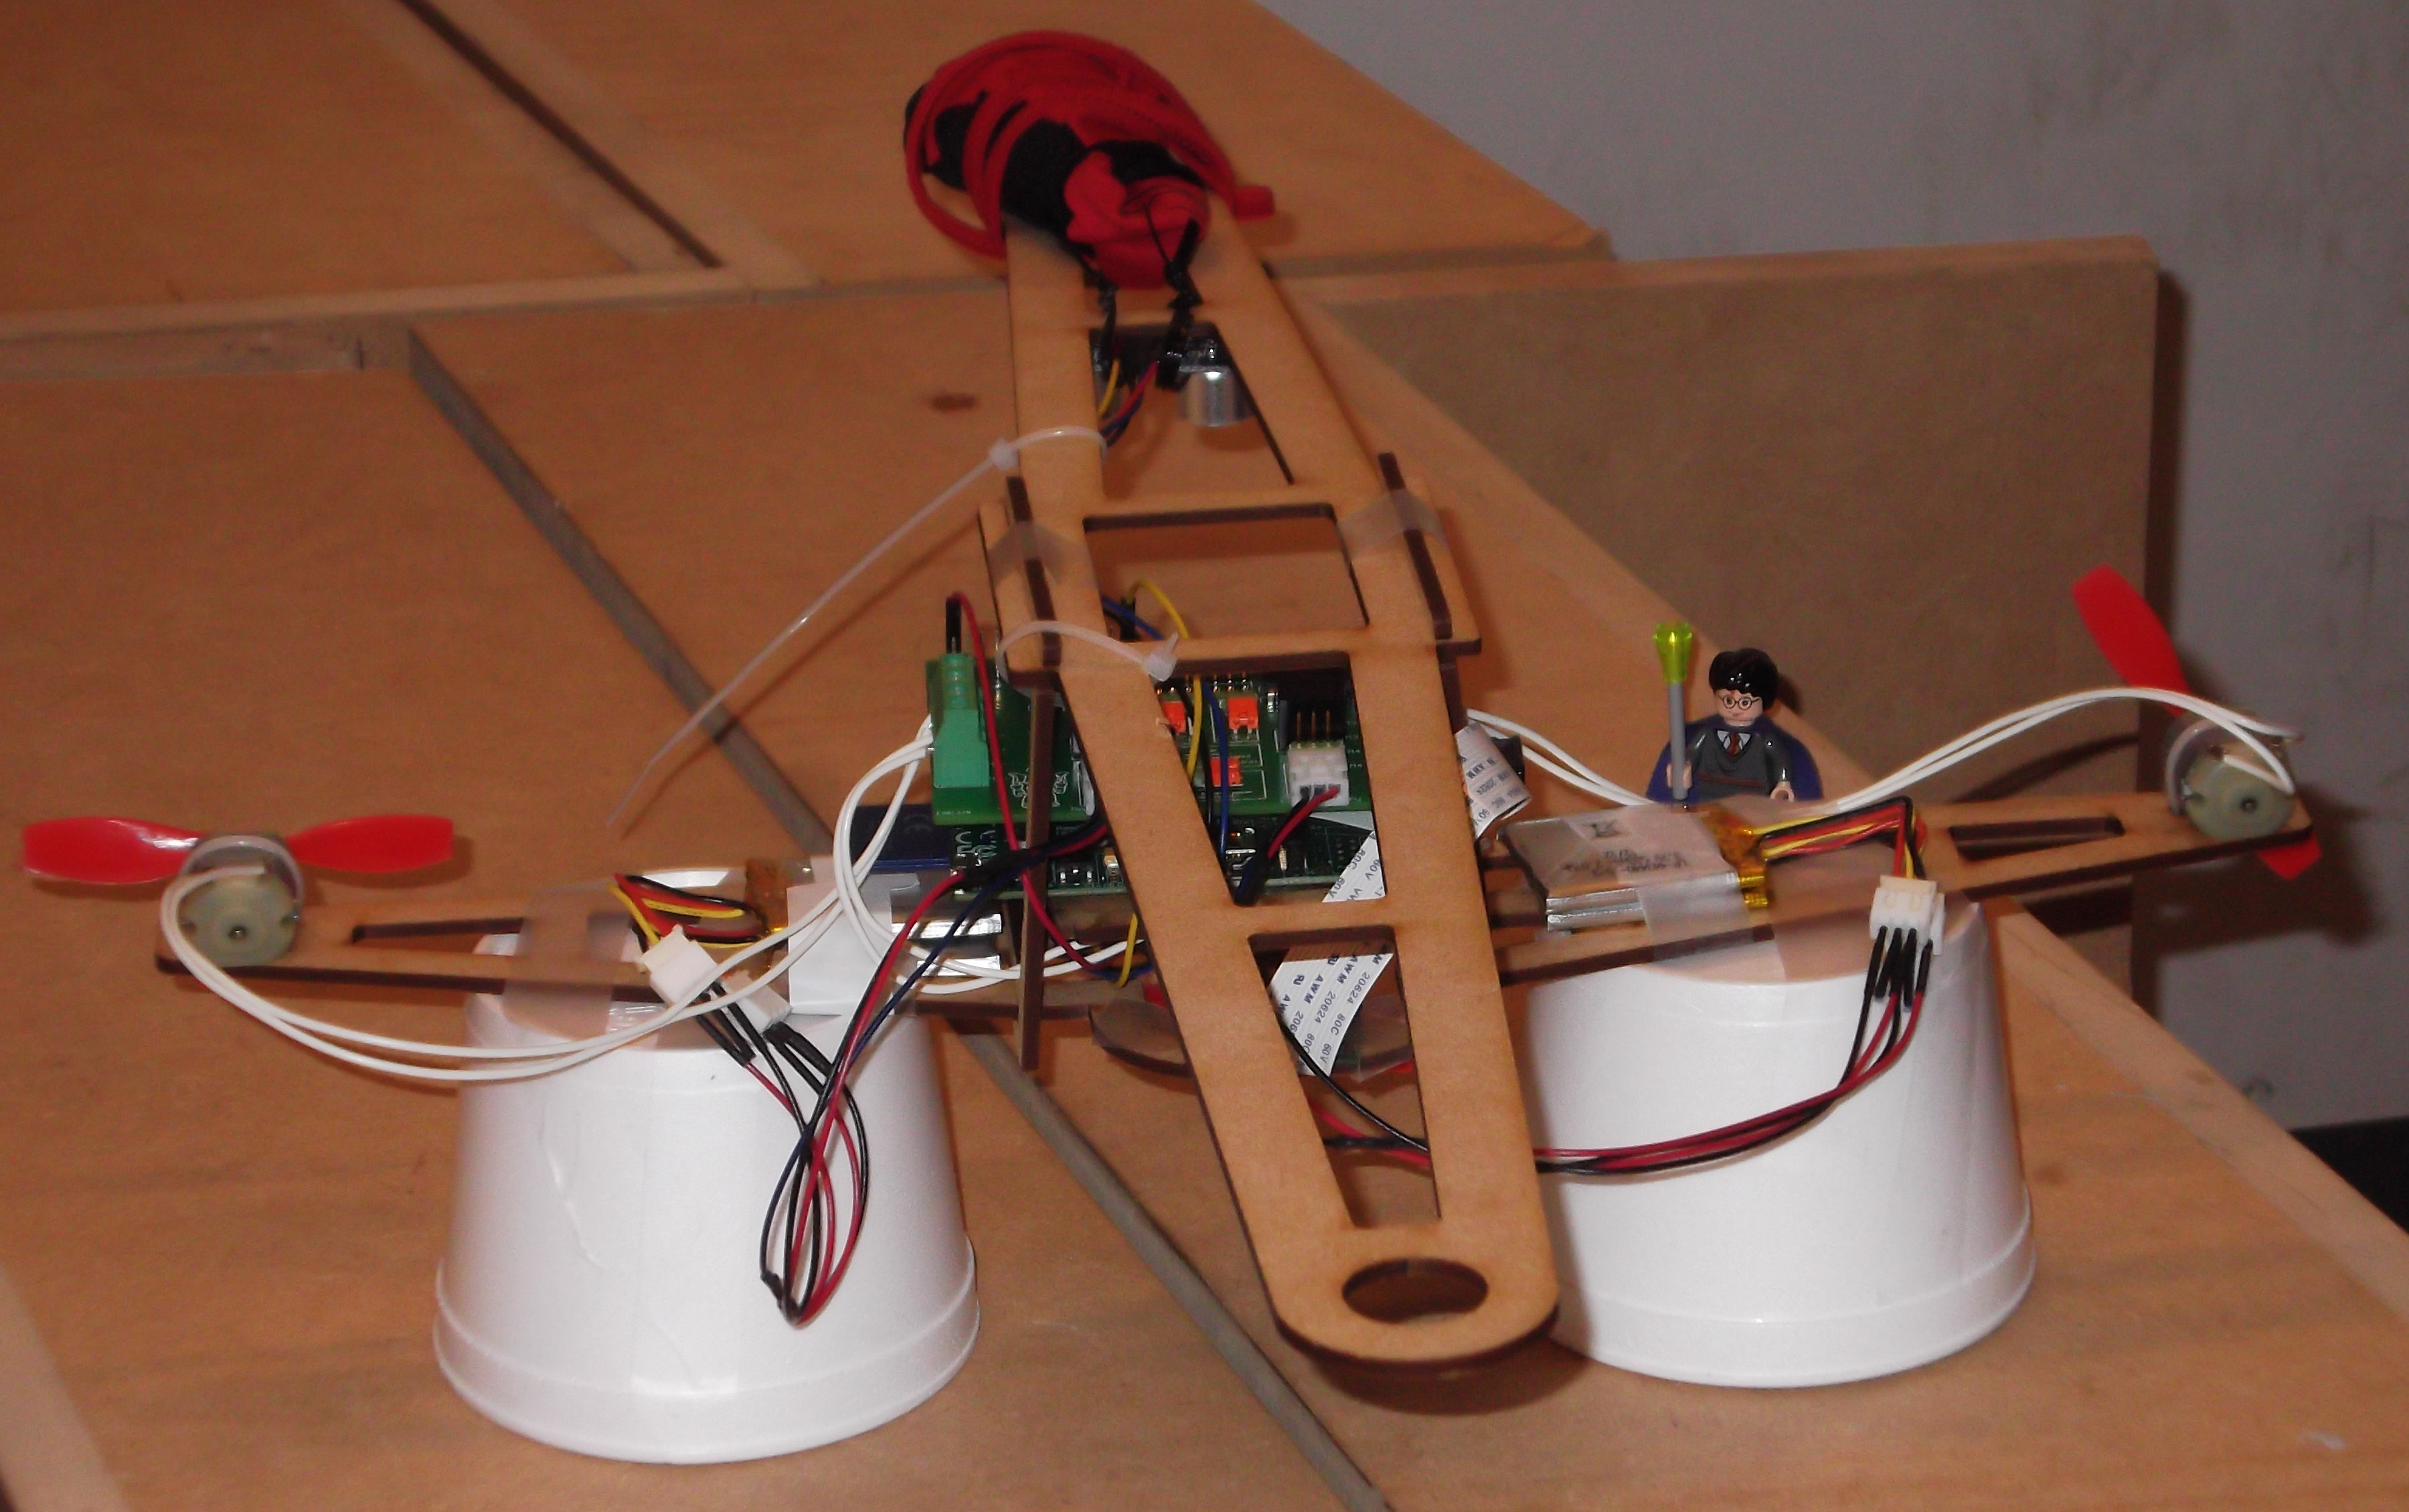
\includegraphics[height=60mm]{zeppelinFrame.jpg}
\caption{Frame met gemonteerde onderdelen}
\label{zeppFrame}
\end{figure}

Om het geheel te monteren, hebben we gebruik gemaakt van plakband en zipties (bundelbandjes). We hebben bekertjes bevestigd om ballast te dragen, zodat het geheel lichtjes zakt wanneer de motor geen kracht naar boven zet. Als gewicht gebruiken we zout, zodat het mogelijk is om nauwkeurig het gewicht te regelen. \\

% == Testen == %
\section{Testen}

Om er zeker van te kunnen zijn dat het aansturen van de zeppelin correct gebeurt, is het nodig dat de componenten getest worden. In deze sectie volgt hierover meer informatie.

\subsection{Afstandssensor}
Voor gedetailleerde gegevens verwijzen we naar het verslag onze zeppelin van het eerste semester (versie 2). Hier hadden we gemerkt dat een enkele waarde van de sensor niet noodzakelijk de correcte afstand weergeeft. Daarom houdt de afstandssensor de laatste 10 gemeten waardes bij. De huidige hoogte wordt gegeven als het gemiddelde van deze waardes (rolling median techniek). Het interval tussen twee metingen hebben we kunnen terugbrengen tot 20 ms.

\subsection{Camera en image processing}


\subsection{Motoren}
In het eerste semester hebben we uitgebreide testen gedaan over de testen en de mogelijkheden van pwm. Het werd duidelijk dat het nodig ging zijn om constant de hoogte te controleren en bij te sturen. Daarnaast bleek ook dat horizontale bewegingen moeilijk exact kunnen worden uitgevoerd, omdat de zeppelin zeer gevoelig is voor allerlei veranderingen van de windomstandigheden in de omgeving: een andere zeppelin die beweegt, de airco, \ldots. 

% == ALGORITMES == %
\section{Algoritmes}
ALGORITME
\subsection{Verticale bewegingen}
Om naar een bepaalde hoogte te stijgen, maken we gebruik van een PID-algoritme\footnote{http://www.csimn.com/CSI\_pages/PIDforDummies.html}. Hierbij gaan we op basis van de huidige fout in hoogte, bepalen of de zeppelin moet stijgen of dalen en met welke kracht. Daarnaast wordt rekening gehouden met de afgeleide, om toekomstige veranderingen te voorspellen. Tenslotte is er de integraal, die fouten uit het verleden voorstelt. Op basis hiervan wordt een pwm-waarde voor de motor gegeven. Het algoritme wordt aangepast aan het gewicht van onze zeppelin en de kracht van de gegeven motoren. \\
De output wordt berekend op basis van deze formule:

\begin{center}
\texttt{output = Kp*error + Ki*integral + Kd*derivative}\\
\end{center}

Hierin zijn Kp, Ki en Kd constanten die we hebben moeten bepalen. Eerst hadden we enkel rekening gehouden met de huidige error (Ki = Kd = 0), maar dit bleek er voor te zorgen dat de zeppelin veel te snel naar een bepaalde hoogte gaat en er dan ver boven of onder gaat. We hebben dit opgelost door Kd te verhogen. Door deze groot te maken, gaat de zeppelin veel rustiger naar de opgegeven hoogte en gaat hij er niet voorbij. Bij de start van het tweede semester hebben we de waardes van deze constanten opnieuw getuned, aangezien er nieuwe volle ballonnen gegeven waren. \\

Er is een HeightController die dit PID-algoritme implementeert, en die er voor gaat zorgen dat de zeppelin zijn hoogte behoudt of naar een gevraagde hoogte gaat. Deze gaat om de 0.1 s de hoogte controleren en de pwm-waarde bijsturen. \\

\subsection{Horizontale bewegingen}
Voor bewegingen in het horizontale vlak maken we eveneens gebruik van een PID-gebaseerd algoritme. Hiervoor zijn er twee afzonderlijke algoritmes die tegelijk lopen (voor de x- en y-richting). Er wordt gebruik gemaakt van de huidige positie van de zeppelin, de co\"{o}rdinaten van de bestemming, en de rotatie van de zeppelin. De positie en rotatie zijn af te leiden van de gegevens die de camera doorstuurt. De verwerking van die gegevens leidt tot de benodigde co\"{o}rdinaten.

% == SOFTWARE == %
\section{Software}

Alle software voor dit project is in Java geschreven. Dit is gekozen omdat dit voor het hele team de meest gebruikte programmeertaal was. Dit gaf wel een verschillende moeilijkheden bij het implementeren van een aantal aspecten (image recognition, \ldots). 

TODO!! afbeelding

\textbf{GUI} \\
De Graphical User Interface stelt de gebruiker in staat om vanaf een client-pc verbinding te maken met de server die het speelveld en de zeppelins controleert. De GUI geeft dan informatie weer over het speelveld en de co\"{o}rdinaten van de zeppelingss.  \\

De eerste tab (`overview') toont de hoogte van beide zeppelins, alsook de toestand van de eigen propellers. Een kaart geeft de locaties van de zeppelings weer. Daarnaast wordt de opdracht van de zeppelins getoond en is er een overzicht van de laatste berichten die zijn uitgewisseld tussen de client en de zeppelin. \\

De tweede tab geeft een uitgebreider overzicht van alle informatie die wordt uitgewisseld tussen de GUI en zeppelin, met een indicatie van de tijd. Er is een mogelijkheid om berichten te filteren op type. \\

\textbf{Image recognition}\\
Voor het tweede deel van de opdracht was er een vorm van image recognition. Hiervoor hebben we gebruik gemaakt van de Java-library OpenCV. Hiermee kan detectie van vormen en kleuren worden ge\"{i}mplementeerd. \\

\textbf{Connectie}\\
 Ook de verbinding is helemaal veranderd in het tweede deel van de opdracht. De twee zeppelins moeten nu communiceren via een server. Die maakt gebruik van de RabbitMQ library.\footnote{https://www.rabbitmq.com/}
\\





% == BESLUIT == %
\section{Besluit}



% == APPENDICES == %
\newpage\makeappendix

\section{Beschrijving van het proces}
Dit onderdeel maakt geen deel uit van dit verslag.


\section{Beschrijving van de werkverdeling}

Hieronder is een tabel te vinden met de gewerkte uren binnen en buiten de sessies: \\

\begin{tabular}{r||r|r|r|r|r}
Overzicht: & Dimitri Jonckers & Wander Bavin & Wout Vekemans & Sunil Tandan & Vince Goossens \\
\hline \hline
09/02 - 15/02 &  &  &  &  &  \\
\hline \hline
Totaal &  &  &  &  &  \\
\end{tabular}


\section{Kritische analyse}
Dit onderdeel maakt geen deel uit van dit verslag.


\end{document}
